\documentclass[aspectratio=1610,onlymath]{beamer}
% \documentclass[aspectratio=1610,onlymath,handout]{beamer}

% Macros used by all lectures, but not necessarily by excercises

%%% General setup and dependencies:

% \usetheme[ddcfooter,nosectionnum]{tud}
\usetheme[nosectionnum,pagenum,noheader]{tud}
% \usetheme[nosectionnum,pagenum]{tud}

% Increase body font size to a sane level:
\let\origframetitle\frametitle
% \renewcommand{\frametitle}[1]{\origframetitle{#1}\normalsize}
\renewcommand{\frametitle}[1]{\origframetitle{#1}\fontsize{10pt}{13.2}\selectfont}
\setbeamerfont{itemize/enumerate subbody}{size=\small} % tud defaults to scriptsize!
\setbeamerfont{itemize/enumerate subsubbody}{size=\small}
% \setbeamerfont{normal text}{size=\small}
% \setbeamerfont{itemize body}{size=\small}

\renewcommand{\emph}[1]{\textbf{#1}}

\def\arraystretch{1.3}% Make tables even less cramped vertically

\usepackage[ngerman]{babel}
\usepackage[utf8]{inputenc}
\usepackage[T1]{fontenc}

%\usepackage{graphicx}
\usepackage[export]{adjustbox} % loads graphicx
\usepackage{import}
\usepackage{stmaryrd}
\usepackage[normalem]{ulem} % sout command
% \usepackage{times}
\usepackage{txfonts}

% \usepackage[perpage]{footmisc} % reset footnote counter on each page -- fails with beamer (footnotes gone)
\usepackage{perpage}  % reset footnote counter on each page
\MakePerPage{footnote}

\usepackage{tikz}
\usetikzlibrary{arrows,positioning}
% Inspired by http://www.texample.net/tikz/examples/hand-drawn-lines/
\usetikzlibrary{decorations.pathmorphing}
\pgfdeclaredecoration{penciline}{initial}{
    \state{initial}[width=+\pgfdecoratedinputsegmentremainingdistance,
    auto corner on length=1mm,]{
        \pgfpathcurveto%
        {% From
            \pgfqpoint{\pgfdecoratedinputsegmentremainingdistance}
                      {\pgfdecorationsegmentamplitude}
        }
        {%  Control 1
        \pgfmathrand
        \pgfpointadd{\pgfqpoint{\pgfdecoratedinputsegmentremainingdistance}{0pt}}
                    {\pgfqpoint{-\pgfdecorationsegmentaspect
                     \pgfdecoratedinputsegmentremainingdistance}%
                               {\pgfmathresult\pgfdecorationsegmentamplitude}
                    }
        }
        {%TO 
        \pgfpointadd{\pgfpointdecoratedinputsegmentlast}{\pgfpoint{1pt}{1pt}}
        }
    }
    \state{final}{}
}
\tikzset{handdrawn/.style={decorate,decoration=penciline}}
\tikzset{every shadow/.style={fill=none,shadow xshift=0pt,shadow yshift=0pt}}
% \tikzset{module/.append style={top color=\col,bottom color=\col}}

% Use to make Tikz attributes with Beamer overlays
% http://tex.stackexchange.com/a/6155
\tikzset{onslide/.code args={<#1>#2}{%
  \only<#1| handout:0>{\pgfkeysalso{#2}} 
}}
\tikzset{onslideprint/.code args={<#1>#2}{%
  \only<#1>{\pgfkeysalso{#2}} 
}}

%%% Title -- always set this first

\newcommand{\defineTitle}[3]{
	\newcommand{\lectureindex}{#1}
	\title{Formale Systeme}
	\subtitle{\href{\lectureurl}{#1. Vorlesung: #2}}
	\author{\href{http://korrekt.org/}{Markus Kr\"{o}tzsch}}
%	\author{\href{http://www.sebastian-rudolph.de}{Sebastian Rudolph} in Vertretung von \href{http://korrekt.org/}{Markus Kr\"{o}tzsch}}
	\date{#3}
	\datecity{TU Dresden}
% 	\institute{Computational Logic}
}

%%% Table of contents:

\RequirePackage{ifthen}

\newcommand{\highlight}[2]{%
	\ifthenelse{\equal{#1}{\lectureindex}}{\alert{#2}}{#2}%
}

\def\myspace{-0.7ex}
\newcommand{\printtoc}{
\begin{tabular}{r@{$\quad$}l}
\highlight{1}{1.} & \highlight{1}{Willkommen/Einleitung formale Sprachen}\\[\myspace]
\highlight{2}{2.} & \highlight{2}{Grammatiken und die Chomsky-Hierarchie}\\[\myspace]
\highlight{3}{3.} & \highlight{3}{Endliche Automaten}\\[\myspace]
\highlight{4}{4.} & \highlight{4}{Complexity of FO query answering}\\[\myspace]
\highlight{5}{5.} & \highlight{5}{Conjunctive queries}\\[\myspace]
\highlight{6}{6.} & \highlight{6}{Tree-like conjunctive queries}\\[\myspace]
\highlight{7}{7.} & \highlight{7}{Query optimisation}\\[\myspace]
\highlight{8}{8.} & \highlight{8}{Conjunctive Query Optimisation / First-Order~Expressiveness}\\[\myspace]
\highlight{9}{9.} & \highlight{9}{First-Order~Expressiveness / Introduction to Datalog}\\[\myspace]
\highlight{10}{10.} & \highlight{10}{Expressive Power and Complexity of Datalog}\\[\myspace]
\highlight{11}{11.} & \highlight{11}{Optimisation and Evaluation of Datalog}\\[\myspace]
\highlight{12}{12.} & \highlight{12}{Evaluation of Datalog (2)}\\[\myspace]
\highlight{13}{13.} & \highlight{13}{Graph Databases and Path Queries}\\[\myspace]
\highlight{14}{14.} & \highlight{14}{Outlook: database theory in practice}
\end{tabular}
}

\newcommand{\overviewslide}{%
\begin{frame}\frametitle{Overview}
\printtoc
\medskip

Siehe \href{\lectureurl}{course homepage [$\Rightarrow$ link]} for more information and materials
\end{frame}
}

%%% Colours:

\usepackage{xcolor,colortbl}
\definecolor{redhighlights}{HTML}{FFAA66}
\definecolor{lightblue}{HTML}{55AAFF}
\definecolor{lightred}{HTML}{FF5522}
\definecolor{lightpurple}{HTML}{DD77BB}
\definecolor{lightgreen}{HTML}{55FF55}
\definecolor{darkred}{HTML}{CC4411}
\definecolor{darkblue}{HTML}{176FC0}%{1133AA}
\definecolor{nightblue}{HTML}{2010A0}%{1133AA}
\definecolor{alert}{HTML}{176FC0}
\definecolor{darkgreen}{HTML}{36AB14}
\definecolor{strongyellow}{HTML}{FFE219}
\definecolor{devilscss}{HTML}{666666}

\newcommand{\redalert}[1]{\textcolor{darkred}{#1}}

%%% Style commands

\newcommand{\quoted}[1]{\texttt{"}{#1}\texttt{"}}
\newcommand{\squote}{\texttt{"}} % straight quote
\newcommand{\Sterm}[1]{\ensuremath{\mathtt{\textcolor{purple}{#1}}}}    % letters in alphabets
\newcommand{\Snterm}[1]{\textsf{\textcolor{darkblue}{#1}}} % nonterminal symbols
\newcommand{\Sntermsub}[2]{\Snterm{#1}_{\Snterm{#2}}} % nonterminal symbols
\newcommand{\Slang}[1]{\textbf{\textcolor{black}{#1}}}    % languages
\newcommand{\Slangsub}[2]{\Slang{#1}_{\Slang{#2}}}    % languages
% Code
\newcommand{\Scode}[1]{\textbf{#1}}    % reserved words in program listings, e.g., "if"
\newcommand{\Scodelit}[1]{\textcolor{purple}{#1}}    % literals in program listings, e.g., strings
\newcommand{\Scomment}[1]{\textcolor{gray}{#1}}    % comment in program listings

\newcommand{\epstrastar}{\mathrel{\mathord{\stackrel{\epsilon}{\to}}{}^*}} % transitive reflexive closure of epsilon transitions in an epslion-NFA

\newcommand{\narrowcentering}[1]{\mbox{}\hfill#1\hfill\mbox{}}

\newcommand{\defeq}{\mathrel{:=}}

\newcommand{\Smach}[1]{\ensuremath{\mathcal{#1}}}    % machines

%%% Slide layout commands:

\newcommand{\sectionSlide}[1]{
\frame{\begin{center}
\LARGE
#1
\end{center}}
}
\newcommand{\sectionSlideNoHandout}[1]{
\frame<handout:0>{\begin{center}
\LARGE
#1
\end{center}}
}

\newcommand{\mydualbox}[3]{%
 \begin{minipage}[t]{#1}
 \begin{beamerboxesrounded}[upper=block title,lower=block body,shadow=true]%
    {\centering\usebeamerfont*{block title}#2}%
    \raggedright%
    \usebeamerfont{block body}
%     \small
    #3%
  \end{beamerboxesrounded}
  \end{minipage}
}
% 
\newcommand{\myheaderbox}[2]{%
 \begin{minipage}[t]{#1}
 \begin{beamerboxesrounded}[upper=block title,lower=block title,shadow=true]%
    {\centering\usebeamerfont*{block title}\rule{0pt}{2.6ex} #2}%
  \end{beamerboxesrounded}
  \end{minipage}
}

\newcommand{\mycontentbox}[2]{%
 \begin{minipage}[t]{#1}%
 \begin{beamerboxesrounded}[upper=block body,lower=block body,shadow=true]%
    {\centering\usebeamerfont*{block body}\rule{0pt}{2.6ex}#2}%
  \end{beamerboxesrounded}
  \end{minipage}
}

\newcommand{\mylcontentbox}[2]{%
 \begin{minipage}[t]{#1}%
 \begin{beamerboxesrounded}[upper=block body,lower=block body,shadow=true]%
    {\flushleft\usebeamerfont*{block body}\rule{0pt}{2.6ex}#2}%
  \end{beamerboxesrounded}
  \end{minipage}
}

% label=180:{\rotatebox{90}{{\footnotesize\textcolor{darkgreen}{Beispiel}}}}
% \hspace{-8mm}\ghost{\raisebox{-7mm}{\rotatebox{90}{{\footnotesize\textcolor{darkgreen}{Beispiel}}}}}\hspace{8mm}
\newcommand{\examplebox}[1]{%
	\begin{tikzpicture}[decoration=penciline, decorate]
		\pgfmathsetseed{1235}
		\node (n1) [decorate,draw=darkgreen, fill=darkgreen!10,thick,align=left,text width=\linewidth, inner ysep=2mm, inner xsep=2mm] at (0,0) {#1};
% 		\node (n2) [align=left,text width=\linewidth,inner sep=0mm] at (n1.92) {{\footnotesize\raisebox{3mm}{\textcolor{darkgreen}{Beispiel}}}};
% 		\node (n2) [decorate,draw=darkgreen, fill=darkgreen!10,thick, align=left,text width=\linewidth,inner sep=2mm] at (n1.90) {{\footnotesize\raisebox{0mm}{\textcolor{darkgreen}{Beispiel}}}};
	\end{tikzpicture}%
}%

\newcommand{\codebox}[1]{%
	\begin{tikzpicture}[decoration=penciline, decorate]
		\pgfmathsetseed{1236}
		\node (n1) [decorate,draw=strongyellow, fill=strongyellow!10,thick,align=left,text width=\linewidth, inner ysep=2mm, inner xsep=2mm] at (0,0) {#1};
	\end{tikzpicture}%
}%

\newcommand{\defbox}[1]{%
	\begin{tikzpicture}[decoration=penciline, decorate]
		\pgfmathsetseed{1237}
		\node (n1) [decorate,draw=darkred, fill=darkred!10,thick,align=left,text width=\linewidth, inner ysep=2mm, inner xsep=2mm] at (0,0) {#1};
	\end{tikzpicture}%
}%

\newcommand{\theobox}[1]{%
	\begin{tikzpicture}[decoration=penciline, decorate]
		\pgfmathsetseed{1240}
		\node (n1) [decorate,draw=darkblue, fill=darkblue!10,thick,align=left,text width=\linewidth, inner ysep=2mm, inner xsep=2mm] at (0,0) {#1};
	\end{tikzpicture}%
}%

\newcommand{\anybox}[2]{%
	\begin{tikzpicture}[decoration=penciline, decorate]
		\pgfmathsetseed{1240}
		\node (n1) [decorate,draw=#1, fill=#1!10,thick,align=left,text width=\linewidth, inner ysep=2mm, inner xsep=2mm] at (0,0) {#2};
	\end{tikzpicture}%
}%


\newsavebox{\mybox}%
\newcommand{\doodlebox}[2]{%
\sbox{\mybox}{#2}%
	\begin{tikzpicture}[decoration=penciline, decorate]
		\pgfmathsetseed{1238}
		\node (n1) [decorate,draw=#1, fill=#1!10,thick,align=left,inner sep=1mm] at (0,0) {\usebox{\mybox}};
	\end{tikzpicture}%
}%

% Common notation

\usepackage{amsmath,amssymb,amsfonts}
\usepackage{xspace}

\newcommand{\lectureurl}{https://iccl.inf.tu-dresden.de/web/FS2016}

\DeclareMathAlphabet{\mathsc}{OT1}{cmr}{m}{sc} % Let's have \mathsc since the slide style has no working \textsc

% Dual of "phantom": make a text that is visible but intangible
\newcommand{\ghost}[1]{\raisebox{0pt}[0pt][0pt]{\makebox[0pt][l]{#1}}}

\newcommand{\tuple}[1]{\langle{#1}\rangle}

%%% Annotation %%%

\usepackage{color}
\newcommand{\todo}[1]{{\tiny\color{red}\textbf{TODO: #1}}}



%%% Old macros below; move when needed

\newcommand{\blank}{\text{\textvisiblespace}} % empty tape cell for TM

% table syntax
\newcommand{\dom}{\textbf{dom}}
\newcommand{\adom}{\textbf{adom}}
\newcommand{\dbconst}[1]{\texttt{"#1"}}
\newcommand{\pred}[1]{\textsf{#1}}
\newcommand{\foquery}[2]{#2[#1]}
\newcommand{\ground}[1]{\textsf{ground}(#1)}
% \newcommand{\foquery}[2]{\{#1\mid #2\}} %% Notation as used in Alice Book
% \newcommand{\foquery}[2]{\tuple{#1\mid #2}}

\newcommand{\quantor}{\mathord{\reflectbox{$\text{\sf{Q}}$}}} % the generic quantor

% logic syntax
\newcommand{\Inter}{\mathcal{I}} %used to denote an interpretation
\newcommand{\Jnter}{\mathcal{J}} %used to denote another interpretation
\newcommand{\Knter}{\mathcal{K}} %used to denote yet another interpretation
\newcommand{\Zuweisung}{\mathcal{Z}} %used to denote a variable assignment

% query languages
\newcommand{\qlang}[1]{{\sf #1}} % Font for query languages
\newcommand{\qmaps}[1]{\textbf{QM}({\sf #1})} % Set of query mappings for a query language

%%% Complexities %%%

\hyphenation{Exp-Time} % prevent "Ex-PTime" (see, e.g. Tobies'01, Glimm'07 ;-)
\hyphenation{NExp-Time} % better that than something else

% \newcommand{\complclass}[1]{{\sc #1}\xspace} % font for complexity classes
\newcommand{\complclass}[1]{\ensuremath{\mathsc{#1}}\xspace} % font for complexity classes

\newcommand{\ACzero}{\complclass{AC$_0$}}
\newcommand{\LogSpace}{\complclass{L}}
\newcommand{\NLogSpace}{\complclass{NL}}
\newcommand{\PTime}{\complclass{P}}
\newcommand{\NP}{\complclass{NP}}
\newcommand{\coNP}{\complclass{coNP}}
\newcommand{\PH}{\complclass{PH}}
\newcommand{\PSpace}{\complclass{PSpace}}
\newcommand{\NPSpace}{\complclass{NPSpace}}
\newcommand{\ExpTime}{\complclass{ExpTime}}
\newcommand{\NExpTime}{\complclass{NExpTime}}
\newcommand{\ExpSpace}{\complclass{ExpSpace}}
\newcommand{\TwoExpTime}{\complclass{2ExpTime}}
\newcommand{\NTwoExpTime}{\complclass{N2ExpTime}}
\newcommand{\ThreeExpTime}{\complclass{3ExpTime}}
\newcommand{\kExpTime}[1]{\complclass{#1ExpTime}}
\newcommand{\kExpSpace}[1]{\complclass{#1ExpSpace}}


% \usetikzlibrary{shapes}

\defineTitle{18}{Turingmaschinen}{7. Januar 2021}

\begin{document}

\maketitle

% \begin{frame}\frametitle{}
% 
% ~\hfill
% \includegraphics[height=6.5cm]{a4}
% \hfill~
% 
% \end{frame}

\sectionSlideNoHandout{Rückblick}

\begin{frame}\frametitle{Zusammenfassung Typ 2}

Kontextfreie Sprachen
\begin{itemize}
\item Beschrieben durch \alert{kontextfreie Grammatiken} und \alert{Kellerautomaten}
\item Können \alert{mehrdeutig} sein
\item Können \alert{deterministisch} sein (beschrieben durch deterministische Kellerautomaten und $\Slang{LR}(k)$-Grammatiken)
\item Wortproblem polynomiell, im deterministischen Fall sogar linear
\item Sonstige Entscheidungsprobleme meist viel schwerer als bei regulären Sprachen 
\item Nicht unter allen Operationen abgeschlossen
\end{itemize}

\end{frame}

\sectionSlide{Turingmaschinen}

\begin{frame}\frametitle{Kellerautomaten erweitern}

Unmittelbar denkbare Erweiterungen von Kellerautomaten:
\begin{itemize}
\item Verwendung von zwei oder mehr Kellern
\item Verwendung von FIFO-Speichern (Warteschlange)
\item Verwendung einer endlichen Menge von Zählern
\item \ldots
\end{itemize}
\alert{All diese Modelle erkennen genau die Typ-0-Sprachen!}
\medskip\pause

Das klassische Automatenmodell\\für diese Sprachklasse ist die \redalert{Turingmaschine}.%
\ghost{\hspace{1.6cm}\raisebox{-0.5cm}{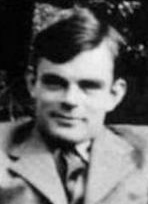
\includegraphics[width=2.0cm]{images/Turing}}}%
\ghost{\hspace{1.6cm}\raisebox{-0.70cm}{\tiny Alan Turing (publ. dom.)}}
\medskip\pause

Was kann diese Art von Automaten?\pause\\
Alles, was überhaupt auf Computern machbar ist!\medskip

\anybox{purple}{\emph{Church-Turing-These:} Die Turingmaschine kann alle Funktionen berechnen,\\
die intuitiv berechenbar sind.}

\end{frame}

\begin{frame}\frametitle{Turingmaschinen -- Grundideen}

\emph{Wesentliche Designentscheidungen}\\
bei der Gestaltung von Turingmaschinen (TMs)\pause:
\begin{itemize}
\item TMs haben eine \alert{endliche Steuerung} (wie bei NFA und PDA)\pause
\item Es gibt eine \alert{unbeschränkte Menge an Speicher} (wie bei PDA)\pause
\item Die TM kann in jedem Schritt \alert{ein Zeichen} aus dem Speicher \alert{lesen} und eines \alert{schreiben} (wie bei PDA)\pause
\item Der Lese-/Schreibzugriff ist \alert{an jeder beliebigen Speicheradresse} möglich\\ (im Gegensatz zu PDA)\\[1ex]

Zur praktischen Implementierung speichert die TM die aktuelle Adresse und kann diese in jedem
Schritt um eins erhöhen oder verringern\pause
\item Zur Vereinfachung wird die Eingabe einfach beim Start in den Speicher übergeben, so dass 
"`Lesen der Eingabe"' und "`Lesen aus Speicher"' die selbe Operation sind
\end{itemize}

\end{frame}

\begin{frame}\frametitle{Turingmaschinen -- Grundideen (2)}

\emph{Schematische Darstellung:}\medskip

\narrowcentering{%
\begin{tikzpicture}[
	scale=0.50,
	decoration=penciline, decorate
]
% \path[use as bounding box] (-3.2,0) rectangle (3.5,-5); % add "draw" to see it
% \draw[help lines] (0,0) grid (5,5);
\pgfmathsetseed{5712}
%
\node (inlabel) [rectangle,draw=none,inner sep=1pt] at (3,0.5) {\alert{Eingabe-/Speicherband}};
\draw[decorate,line width=0.3mm] (-1,0) -- (10.5,0);
\draw[decorate,line width=0.3mm] (-1,-1) -- (10.5,-1);
\foreach \x in {0,...,10} {
	\draw[decorate,line width=0.3mm] (\x-1,0) -- (\x-1,-0.9);
	\node (s\x) [circle,draw=none,inner sep=1pt] at (\x-0.5,-0.5) {\ifthenelse{\x<5}{\ifthenelse{\x<3}{\Sterm{a}}{\Sterm{b}}}{\ifthenelse{\x=5 \OR \x=7 \OR \x=8}{\Snterm{C}}{\ifthenelse{\x=9}{\Sterm{b}}{\Snterm{D}}}}};
}
\draw[decorate,line width=0.3mm] (10,0) -- (10,-0.9);
\node (dots) [circle,draw=none,inner sep=1pt] at (11.1,-0.5) {$\cdots$};

% \draw[decorate,line width=0.3mm] (5.5,0) -- (6,0) -- (6,-0.9) -- (5.5,-0.9) ;
% \draw[decorate,line width=0.3mm] (6,0) -- (6,-0.9);

\draw[fill=none,decorate,line width=0.3mm]
	(2,-3) -- (6,-3) -- (6,-7) -- (2,-7) -- cycle;
\node (falabel) [circle,draw=none,inner sep=1pt,align=left] at (4,-5) {Endliche\\Steuerung};
\draw[fill=none,decorate,line width=0.4mm,darkblue,->]
	(4,-3) -- (4,-2) -- (6.5,-2) -> (6.5,-1);
\node (headlabel) [rectangle,draw=none,inner sep=1pt,align=left] at (9.5,-2.0) {\footnotesize\alert{Lese-/Schreibkopf}\\[-0.6ex]\footnotesize\alert{(beweglich)}};

\node[rectangle,align=center,draw,line width=0.3mm,decorate, minimum width=8mm, minimum height=8mm] (state) at (8, -6) {$q$};
\draw[fill=none,decorate,line width=0.4mm,darkblue,->]
	(6,-6) -> (state.180);
\node (qlabel) [rectangle,draw=none,inner sep=1pt] at (11.5,-6) {\footnotesize\alert{Zustandsvariable}};

% \node[cloud, cloud puffs=15.7, cloud ignores aspect, minimum width=4cm, minimum height=1cm, align=center, draw,line width=0.3mm] (memory) at (11, -1) {\alert{zusätzlicher}\\\alert{Speicher}};
% 
% \draw[fill=none,decorate,line width=0.3mm] (9,0) -- (14,0);
% \draw[fill=none,decorate,line width=0.3mm] (9,-1) -- (14,-1);
% \draw[fill=none,decorate,line width=0.3mm] (9,0) -- (9,-1);
% \foreach \y in {10,...,14} {
% 	\draw[fill=none,decorate,line width=0.3mm] (\y,0) -- (\y,-0.9);
% 	\node (k\y) [circle,draw=none,inner sep=1pt] at (\y-0.5,-0.5) {\ifthenelse{\y<12}{\Snterm{A}}{\Snterm{B}}};
% }
% \draw[fill=none,decorate,line width=0.4mm,darkblue,->]
% 	(6,-3.5) -- (7.5,-3.5) -- (7.5,-0.5) -> (9,-0.5);
% \node (stacklabel) [circle,draw=none,inner sep=1pt] at (11.5,-1.5) {\alert{Warteschlange}};
\end{tikzpicture}}
\bigskip\pause

\emph{Übergangsfunktion:}
\begin{itemize}
\item \alert{Eingabe:} aktueller Zustand, gelesenes Zeichen
\item \alert{Ausgabe:} neuer Zustand, geschriebenes Zeichen, Änderung Lese-/Schreibadresse (${}\hat{=}{}$ Bewegung Lese-/Schreibkopf)
\end{itemize}

\end{frame}

\begin{frame}\frametitle{Speicherzugriff in TMs}


\alert{Speicherverwaltung:}
\begin{itemize}
\item Zu jedem Zeitpunkt verwendet die TM endlich viele Speicherzellen
\item Speicherzellen als "`Band"' von links nach rechts
\item Lese-/Schreibkopf kann frei auf Band bewegt werden (pro Schritt um eine Zelle nach links oder rechts)
\item Am linken Rand kann der Kopf nicht weiter nach links bewegt werden
\item Am rechten Rand des Speichers kann der Kopf nach rechts bewegt werden: dann wird dort eine neue Speicherzelle mit dem Inhalt $\blank$ (Leerzeichen, Blank) angefügt
\end{itemize}\bigskip

\alert{Alternative Vorstellung:} Der Speicher ist ein einseitig unendlich langes Band, auf dem am Anfang nur
eine (endliche) Eingabe steht, gefolgt von unendlich vielen leeren Zellen \ghost{($\blank$).}


\end{frame}

\begin{frame}

\narrowcentering{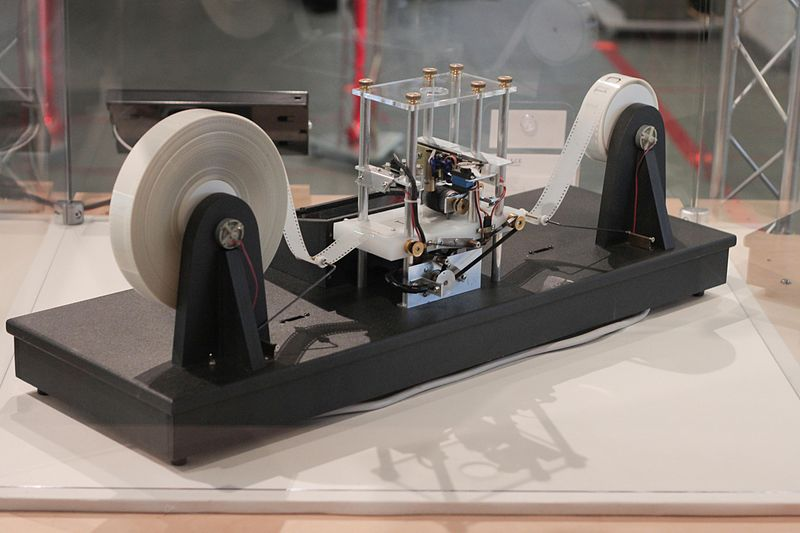
\includegraphics[width=9.9cm]{images/TM}}

\narrowcentering{\tiny Modell einer Turingmaschine, (c) Foto: Rocky Acosta, 2012, CC-By 3.0}
\end{frame}

\begin{frame}\frametitle{Definition TM}

\defbox{Eine \redalert{(deterministische) Turingmaschine} (DTM) ist ein Tupel
$\Smach{M}=\tuple{Q,\Sigma,\Gamma,\delta,q_0,F}$ mit
den folgenden Bestandteilen:
\begin{itemize}
\item $Q$: endliche Menge von \redalert{Zuständen}
\item $\Sigma$: \redalert{Eingabealphabet}
\item $\Gamma$: \redalert{Arbeitsalphabet} mit $\Gamma\supseteq\Sigma\cup\{\blank\}$
\item $\delta$: \redalert{Übergangsfunktion}, eine partielle Funktion\\[1ex]
\narrowcentering{$Q\times\Gamma \to Q\times\Gamma\times\{L,R,N\}$}
% , wobei $2^Q$ die Potenzmenge von $Q$ ist
\item $q_0$: \redalert{Startzustand} $q_0\in Q$
\item $F$: Menge von akzeptierenden \redalert{Endzuständen} $F\subseteq Q$
\end{itemize}
}

\alert{Dabei bedeutet $\delta(q,a)=\tuple{p,b,D}$:}\\
\hspace{5mm}"`Liest die TM in Zustand $q$ unter dem Lese-/Schreibkopf ein $a$,\\
\hspace{5.8mm}dann wechselt sie zu Zustand $p$, überschreibt das $a$ mit $b$\\
\hspace{5.8mm}und verschiebt den Lese-/Schreibkopf gemäß $D\in\{L,R,N\}$\\
\hspace{5.8mm}(nach links, nach rechts, gar nicht)."'
% 
% \begin{itemize}
% \item Liest die TM in Zustand $q$ unter dem Lese-/Schreibkopf ein $a$,
% \item dann wechselt sie zu Zustand $p$
% \item überschreibt das $a$ mit $b$
% \item und verschiebt den Lese-/Schreibkopf gemäß $D\in\{L,R,N\}$ (nach links, nach rechts, gar nicht)
% \end{itemize}
% 
% \begin{itemize}
% \item Die Buchstaben $L$, $R$, $N$ geben an, wie der Lese-/Schreibkopf bewegt werden soll
% (nach links, nach rechts, gar nicht)
% \item Die TM hält an, wenn die Übergangsfunktion für die aktuelle Konfiguration nicht definiert ist
% \end{itemize}

\end{frame}

\begin{frame}\frametitle{Beispiel (1)}

Wir konstruieren eine TM mit dem Eingabealphabet $\Sigma=\{\Sterm{0}\}$,\\ welche
Wörter der Sprache $\{\Sterm{0}^{2^i}\mid i\geq 0\}$ akzeptiert\\
(Ketten von $\Sterm{0}$, deren Länge eine Zweierpotenz ist)
\pause\bigskip

\emph{Arbeitsweise:}
\begin{enumerate}[(1)]
\item Laufe von links nach rechts über die Eingabe und ersetze dabei jede zweite $\Sterm{0}$ durch\ghost{ $\Snterm{X}$}
\item Falls insgesamt nur eine $\Sterm{0}$ gefunden wird, akzeptiere
\item Falls eine andere ungerade Zahl an $\Sterm{0}$ gefunden wird, verwirf
\item Laufe zurück zum Anfang des Bandes
\item Wiederhole die Schritte ausgehend von (1)
\end{enumerate}

\end{frame}

\begin{frame}\frametitle{Beispiel (2)}

\emph{Wir können TMs in Diagrammen darstellen:}\medskip

Ein Pfeil $s_1\mapsto s_2,D$ von $q_1$ nach $q_2$ bedeutet $\delta(q_1,s_1)=\tuple{q_2,s_2,D}$
\bigskip\pause

\emph{Übergangsrelation zum Beispiel:}\medskip

\begin{tikzpicture}[baseline={(q1.base)}]
% \draw[help lines] (0,0) grid (7,2);
\node (q1) [circle,draw=black,thick] at (0,0) {$q_0$};
\node (q2) [circle,draw=black,thick] at (3,0) {$q_1$};
\node (q3) [circle,draw=black,thick] at (6,0) {$q_2$};
\node (q4) [circle,draw=black,thick] at (9,0) {$q_3$};
\node (q5) [circle,draw=black,thick] at (4.5,-2) {$q_4$};
\node (q6) [circle,draw=black,thick,double] at (1.5,-2) {$q_5$};
%
\path[->,line width=0.5mm](0,1) edge (q1);
\path[->,line width=0.5mm](q1) edge node[above] {$\Sterm{0}\mapsto\Snterm{$\hat{0}$},R$} (q2);
\path[->,line width=0.5mm](q2) edge node[above] {$\Sterm{0}\mapsto\Snterm{X},R$} (q3);
\path[->,line width=0.5mm,bend left=15](q3) edge node[above] {$\Sterm{0}\mapsto\Sterm{0},R$} (q4);
\path[->,line width=0.5mm,bend left=15](q4) edge node[below] {$\Sterm{0}\mapsto\Snterm{X},R$} (q3);

\path[->,line width=0.5mm](q2) edge [loop above] node[above] {$\Snterm{X}\mapsto\Snterm{X},R$} (q2);
\path[->,line width=0.5mm](q3) edge [loop above] node[above] {$\Snterm{X}\mapsto\Snterm{X},R$} (q3);
\path[->,line width=0.5mm](q4) edge [loop above] node[above] {$\Snterm{X}\mapsto\Snterm{X},R$} (q4);

\path[->,line width=0.5mm,bend left](q3) edge node[right] {$\blank\mapsto\blank,L$} (q5);
\path[->,line width=0.5mm](q5) edge [loop below] node[below,align=left] {$\Snterm{X}\mapsto\Snterm{X},L$\\$\Sterm{0}\mapsto\Sterm{0},L$} (q5);
\path[->,line width=0.5mm,bend left](q5) edge node[right,xshift=-5pt,yshift=7pt] {$\Snterm{$\hat{0}$}\mapsto\Snterm{$\hat{0}$},R$} (q2);

\path[->,line width=0.5mm](q2) edge node[left] {$\blank\mapsto\blank,N$} (q6);
\end{tikzpicture}

\end{frame}

\begin{frame}\frametitle{Arbeitsweise einer TM: Übergänge}

Sei $\Smach{M}=\tuple{Q,\Sigma,\Gamma,\delta,q_0,F}$ eine DTM.

\defbox{Eine \redalert{Konfiguration} von $\Smach{M}$ ist ein Wort
$w\,q\,v\in\Gamma^* \circ Q \circ \Gamma^*$, wobei $w$ den Bandinhalt vor
dem Lese-/Schreibkopf, $q$ den aktuellen Zustand und $v$ den Bandinhalt ab
dem Lese-/Schreibkopf darstellt.
% \medskip
% 
% Wir definieren eine \redalert{Übergangsrelation} zwischen Konfigurationen wie folgt:\smallskip
% 
% Die Konfiguration $waqbv$ kann in die Konfiguration $\tuple{q',w,\psi'\gamma}$ übergehen,
% in Symbolen $\tuple{q,vw,\psi\gamma}\vdash\tuple{q',w,\psi'\gamma}$, 
% falls gilt $\tuple{q',\psi'}\in \delta(q,v,\psi)$.\footnote{\textcolor{devilscss}{Anmerkung: In diesem Fall ist $v\in\Sigma_\epsilon$ und $\psi,\psi'\in\Gamma_\epsilon$.}}
% Mit $\vdash^*$ bezeichnen wir den reflexiven, transitiven Abschluss von $\vdash$.
}\pause

\defbox{Sei $w\,q\,av$ eine Konfiguration, mit $w,v\in\Gamma^*$, $a\in\Gamma$ und $q\in Q$.
Die \redalert{Übergangsrelation $\vdash$} ist wie folgt definiert:
\begin{itemize}
\item Falls $\delta(q,a)=\tuple{r,b,N}$, dann $w\,q\,av\vdash w\,r\,bv$.
\item Falls $\delta(q,a)=\tuple{r,b,R}$ 
\begin{itemize}
\item falls $v\neq\epsilon$, dann $w\,q\,av\vdash wb\,r\,v$;
\item falls $v=\epsilon$, dann $w\,q\,av\vdash wb\,r\,\blank$.
\end{itemize}
% und $v\neq\epsilon$, dann $w\,q\,av\vdash wb\,r\,v$.
% \item Falls $\delta(q,a)=\tuple{r,b,R}$ und $v=\epsilon$, dann $w\,q\,av\vdash wb\,r\,\blank$.
\item Falls $\delta(q,a)=\tuple{r,b,L}$ 
\begin{itemize}
\item falls $w=w'c$ mit $c\in\Gamma$, dann $w\,q\,av\vdash w'\,r\,cbv$;
\item falls $w=\epsilon$, dann $w\,q\,av\vdash r\,bv$.
\end{itemize}
% 
% \item Falls $\delta(q,a)=\tuple{r,b,L}$ und $w=\epsilon$, dann $w\,q\,av\vdash r\,bv$.
\end{itemize}
Mit $\vdash^*$ bezeichnen wir den reflexiven, transitiven Abschluss von $\vdash$.
}

\end{frame}


\begin{frame}\frametitle{Beispiel (3)}

% \emph{Übergangsrelation zum Beispiel:}\medskip

\begin{tikzpicture}[baseline={(q1.base)}]
% \draw[help lines] (0,0) grid (7,2);
\node (q1) [circle,draw=black,thick] at (0,0) {$q_0$};
\node (q2) [circle,draw=black,thick] at (3,0) {$q_1$};
\node (q3) [circle,draw=black,thick] at (6,0) {$q_2$};
\node (q4) [circle,draw=black,thick] at (9,0) {$q_3$};
\node (q5) [circle,draw=black,thick] at (4.5,-2) {$q_4$};
\node (q6) [circle,draw=black,thick,double] at (1.5,-2) {$q_5$};
%
\path[->,line width=0.5mm](0,1) edge (q1);
\path[->,line width=0.5mm](q1) edge node[above] {$\Sterm{0}\mapsto\Snterm{$\hat{0}$},R$} (q2);
\path[->,line width=0.5mm](q2) edge node[above] {$\Sterm{0}\mapsto\Snterm{X},R$} (q3);
\path[->,line width=0.5mm,bend left=15](q3) edge node[above] {$\Sterm{0}\mapsto\Sterm{0},R$} (q4);
\path[->,line width=0.5mm,bend left=15](q4) edge node[below] {$\Sterm{0}\mapsto\Snterm{X},R$} (q3);

\path[->,line width=0.5mm](q2) edge [loop above] node[above] {$\Snterm{X}\mapsto\Snterm{X},R$} (q2);
\path[->,line width=0.5mm](q3) edge [loop above] node[above] {$\Snterm{X}\mapsto\Snterm{X},R$} (q3);
\path[->,line width=0.5mm](q4) edge [loop above] node[above] {$\Snterm{X}\mapsto\Snterm{X},R$} (q4);

\path[->,line width=0.5mm,bend left](q3) edge node[right] {$\blank\mapsto\blank,L$} (q5);
\path[->,line width=0.5mm](q5) edge [loop below] node[right,align=left,xshift=1mm] {$\Snterm{X}\mapsto\Snterm{X},L$\\$\Sterm{0}\mapsto\Sterm{0},L$} (q5);
\path[->,line width=0.5mm,bend left](q5) edge node[right,xshift=-5pt,yshift=7pt] {$\Snterm{$\hat{0}$}\mapsto\Snterm{$\hat{0}$},R$} (q2);

\path[->,line width=0.5mm](q2) edge node[left] {$\blank\mapsto\blank,N$} (q6);
\end{tikzpicture}

\emph{Übergänge bei Eingabe von $\Sterm{0000}$:}\medskip

$q_0\,\Sterm{0000} \pause\vdash \Snterm{$\hat{0}$}\,q_1\,\Sterm{000} \pause\vdash  \Snterm{$\hat{0}$X}\,q_2\,\Sterm{00}\pause\vdash  \Snterm{$\hat{0}$X}\Sterm{0}\,q_3\,\Sterm{0} \pause\vdash \Snterm{$\hat{0}$X}\Sterm{0}\Snterm{X}\,q_2\,\blank \pause\vdash
\Snterm{$\hat{0}$X}\Sterm{0}\,q_4\,\Snterm{X}\blank\pause\vdash{}$\\[1ex]
%
$\Snterm{$\hat{0}$X}\,q_4\,\Sterm{0}\Snterm{X}\blank \vdash\Snterm{$\hat{0}$}\,q_4\,\Snterm{X}\Sterm{0}\Snterm{X}\blank \vdash q_4\,\Snterm{$\hat{0}$}\Snterm{X}\Sterm{0}\Snterm{X}\blank\pause\vdash\Snterm{$\hat{0}$}\,q_1\,\Snterm{X}\Sterm{0}\Snterm{X}\blank\pause\vdash\Snterm{$\hat{0}$}\Snterm{X}\,q_1\,\Sterm{0}\Snterm{X}\blank\pause\vdash\ghost{$\Snterm{$\hat{0}$}\Snterm{X}\Snterm{X}\,q_2\,\Snterm{X}\blank\pause\vdash{}$}$\\[1ex]
%
$\Snterm{$\hat{0}$}\Snterm{X}\Snterm{X}\Snterm{X}\,q_2\,\blank\pause\vdash\Snterm{$\hat{0}$}\Snterm{X}\Snterm{X}\,q_4\,\Snterm{X}\blank\vdash\Snterm{$\hat{0}$}\Snterm{X}\,q_4\,\Snterm{X}\Snterm{X}\blank\vdash\Snterm{$\hat{0}$}\,q_4\,\Snterm{X}\Snterm{X}\Snterm{X}\blank\vdash q_4\,\Snterm{$\hat{0}$}\Snterm{X}\Snterm{X}\Snterm{X}\blank
 \vdash{}$\\[1ex]
%
$\Snterm{$\hat{0}$}\,q_1\,\Snterm{X}\Snterm{X}\Snterm{X}\blank \pause\vdash\Snterm{$\hat{0}$}\Snterm{X}\,q_1\,\Snterm{X}\Snterm{X}\blank\vdash\Snterm{$\hat{0}$}\Snterm{X}\Snterm{X}\,q_1\,\Snterm{X}\blank\vdash\Snterm{$\hat{0}$}\Snterm{X}\Snterm{X}\Snterm{X}\,q_1\,\blank\pause\vdash\Snterm{$\hat{0}$}\Snterm{X}\Snterm{X}\Snterm{X}\,q_5\,\blank$
\end{frame}


\begin{frame}\frametitle{Arbeitsweise einer TM: Läufe}

Für Eingabewort $w$ beginnt die TM mit der \redalert{Startkonfiguration} $q_0\,w$.
\pause\medskip

Ein \redalert{Lauf} ist eine maximale Folge von Konfigurationen, die durch die Übergangsrelation in Beziehung stehen
\begin{itemize}
\item Ein Lauf kann endlich sein, wenn es für die Schlusskonfiguration keinen Nachfolger gibt
\item Ein Lauf kann unendlich sein, wenn immer neue Konfigurationen erreichbar sind
\end{itemize}
\pause\medskip

Die TM \redalert{akzeptiert} die Eingabe, wenn der (eindeutig bestimmte) Lauf, der mit $q_0\,w$ beginnt, endlich ist und seine letzte Konfiguration einen Endzustand beinhaltet.
\medskip

Andernfalls \redalert{verwirft} die TM die Eingabe.
\medskip
% 
% \emph{Anmerkung:} Im Gegensatz zum PDA kann eine TM nur akzeptieren, wenn sie zuvor angehalten hat, d.h., wenn es keine Folgerkonfigurationen mehr gibt.

\end{frame}

\begin{frame}\frametitle{Sprache einer TM}

Die Sprache einer TM wird wie erwartet definiert:

\defbox{Die von einer TM $\Smach{M}$ \redalert{erkannte Sprache} $\Slang{L}(\Smach{M})$ ist die Menge aller Wörter, die von einer TM akzeptiert werden.}\pause

Zwei Gründe für Nichtakzeptanz von Wörtern:
\begin{enumerate}[(1)]
\item TM hält in einem Zustand, der kein Endzustand ist
\item TM hält nicht (Endlosschleife)
\end{enumerate}
Es ist praktisch, wenn eine TM garantiert hält, da man Fall (2) meist nicht sicher erkennen kann (man weiß nicht, ob die TM irgendwann doch noch anhält)

\defbox{Eine TM ist ein \redalert{Entscheider}, wenn sie bei jeder Eingabe hält. Wir sagen in diesem Fall, dass die TM die von ihr erkannte Sprache \redalert{entscheidet}.}

\end{frame}

\begin{frame}\frametitle{Beispiel (4)}

\begin{tikzpicture}[baseline={(q1.base)}]
% \draw[help lines] (0,0) grid (7,2);
\node (q1) [circle,draw=black,thick] at (0,0) {$q_0$};
\node (q2) [circle,draw=black,thick] at (3,0) {$q_1$};
\node (q3) [circle,draw=black,thick] at (6,0) {$q_2$};
\node (q4) [circle,draw=black,thick] at (9,0) {$q_3$};
\node (q5) [circle,draw=black,thick] at (4.5,-2) {$q_4$};
\node (q6) [circle,draw=black,thick,double] at (1.5,-2) {$q_5$};
%
\path[->,line width=0.5mm](0,1) edge (q1);
\path[->,line width=0.5mm](q1) edge node[above] {$\Sterm{0}\mapsto\Snterm{$\hat{0}$},R$} (q2);
\path[->,line width=0.5mm](q2) edge node[above] {$\Sterm{0}\mapsto\Snterm{X},R$} (q3);
\path[->,line width=0.5mm,bend left=15](q3) edge node[above] {$\Sterm{0}\mapsto\Sterm{0},R$} (q4);
\path[->,line width=0.5mm,bend left=15](q4) edge node[below] {$\Sterm{0}\mapsto\Snterm{X},R$} (q3);

\path[->,line width=0.5mm](q2) edge [loop above] node[above] {$\Snterm{X}\mapsto\Snterm{X},R$} (q2);
\path[->,line width=0.5mm](q3) edge [loop above] node[above] {$\Snterm{X}\mapsto\Snterm{X},R$} (q3);
\path[->,line width=0.5mm](q4) edge [loop above] node[above] {$\Snterm{X}\mapsto\Snterm{X},R$} (q4);

\path[->,line width=0.5mm,bend left](q3) edge node[right] {$\blank\mapsto\blank,L$} (q5);
\path[->,line width=0.5mm](q5) edge [loop below] node[right,align=left,xshift=1mm] {$\Snterm{X}\mapsto\Snterm{X},L$\\$\Sterm{0}\mapsto\Sterm{0},L$} (q5);
\path[->,line width=0.5mm,bend left](q5) edge node[right,xshift=-5pt,yshift=7pt] {$\Snterm{$\hat{0}$}\mapsto\Snterm{$\hat{0}$},R$} (q2);

\path[->,line width=0.5mm](q2) edge node[left] {$\blank\mapsto\blank,N$} (q6);
\end{tikzpicture}
\bigskip

Diese TM entscheidet die Sprache $\{\Sterm{0}^{2^i}\mid i\geq 0\}$.

\end{frame}

\begin{frame}\frametitle{Turingmaschinen programmieren}

\emph{Beobachtung:} Die detaillierte Beschreibung von TMs ist in der Regel sehr aufwändig
\bigskip

\emph{Abhilfe:} Oft reicht die skizzenhafte Beschreibung der Arbeitsweise
\medskip\pause

\examplebox{Beispiel: Eine TM zur Erkennung von $\{\Sterm{a}^i\Sterm{b}^i\Sterm{c}^i\mid i\geq 0\}$ arbeitet wie folgt:
\footnotesize
\begin{enumerate}[(1)]
% \item Falls $\blank$ gelesen wird, akzeptiere
\item Ersetze, angefangen von links, Vorkommen von $\Sterm{a}$ durch $\Snterm{$\hat{a}$}$
\item Immer wenn ein $\Sterm{a}$ ersetzt wurde, suche ein $\Sterm{b}$ und ersetze es durch $\Snterm{$\hat{b}$}$,
suche anschließend rechts davon ein $\Sterm{c}$ und ersetze es durch $\Snterm{$\hat{c}$}$
\item Gehe danach zurück zum ersten noch nicht ersetzten $\Sterm{a}$ und führe die Ersetzung (1) fort, bis alle $\Sterm{a}$ ersetzt worden sind
\item Akzeptiere, falls der Inhalt des Bandes die Form $\Snterm{$\hat{a}$}^*\Snterm{$\hat{b}$}^*\Snterm{$\hat{c}$}^*$ hat
\item Andernfalls oder falls eine der Ersetzungen in Schritt (2) fehlschlägt, weil es zu wenige $\Sterm{b}$ oder $\Sterm{c}$ gibt, lehne die Eingabe ab
\end{enumerate}
}

\end{frame}

\begin{frame}\frametitle{Berechnung vs. Worterkennung}

Wir haben TMs als \alert{Automaten zur Worterkennung} definiert:
\begin{itemize}
\item Eingabe wird am Anfang auf Band gegeben
\item TM kann (a) anhalten und die Eingabe akzeptieren, (b) anhalten und die Eingabe ablehnen oder (c) nicht anhalten
\end{itemize}
\bigskip

\alert{Wie kann man TMs als allgemeines Rechenmodell verstehen?}\pause

\begin{enumerate}[(1)]
\item Berechnungsfragen können als Wortproblem kodiert werden.
\begin{itemize}
\item Eingabewörter als Kodierung beliebiger Eingaben (z.B. als Binärdatei)
\item Berechnung einer Booleschen Funktion\\
$\leadsto$ \redalert{Entscheidungsproblem}
\end{itemize}\pause
%
\item Alternative Definition: Der Inhalt des Bandes beim Halten der TM wird als Ausgabe interpretiert (keine Endzustände nötig).\\
Dann kodieren TMs partielle Funktionen $\Sigma^*\to\Gamma^*$ (partiell, da die TM nicht immer anhalten muss)
\end{enumerate}

\end{frame}

\begin{frame}\frametitle{Die Church-Turing-These}

Was ist mit dem intuitiven Begriff der "`mechanisch berechenbaren"' Funktion gemeint?\pause
% \bigskip
% 
\begin{itemize}
\item \alert{Gödel/Herbrand (1934):} allgemeine rekursive Funktionen
\item \alert{Church (1936):} $\lambda$-Kalkül
\item \alert{Turing (1936):} Turingmaschine (ursprünglich "`a-machine"')\pause
\item \alert{Kleene/Rosser/Church/Turing:} Die drei Ansätze beschreiben die gleiche Klasse von Funktionen!
\end{itemize}

\anybox{purple}{\emph{Church-Turing-These:} Eine Funktion ist genau dann im intuitiven Sinne berechenbar, wenn es
eine Turingmaschine gibt, die für jede mögliche Eingabe den Wert der Funktion auf das Band schreibt und anschließend hält.
}\pause

\begin{itemize}
\item \emph{Lesart 1:} Vorschlag einer mathematischen Definition der intuitiven Idee von Berechenbarkeit
\item \emph{Lesart 2:} "`Naturgesetz"' über die Möglichkeiten und Grenzen des Rechnens an sich
\end{itemize}

\end{frame}

\begin{frame}\frametitle{Computer sind kompliziert}

Das Modell der Turingmaschine ist \redalert{einfach}\\
das Verhalten von Turingmaschinen ist es \redalert{nicht!}\bigskip

Betrachten wir einen ganz einfachen Sonderfall:
\begin{itemize}
\item TMs mit nur \alert{fünf Zuständen}
\item und nur \alert{zwei Zeichen} im Bandalphabet
\item bei \alert{Eingabe $\epsilon$} (leeres Wort)
\end{itemize}\pause\bigskip

Bereits diese "`Spielzeugbeispiele"' werden auch 80 Jahre nach Einführung der TM noch nicht völlig verstanden:
\begin{itemize}
\item Es gibt TMs dieser Art, die bei Eingabe $\epsilon$ erst nach über 47 Millionen Übergängen${}^1$ anhalten
\item Es gibt TMs dieser Art, von denen wir bis heute nicht wissen, ob sie bei Eingabe $\epsilon$ jemals anhalten oder nicht
\end{itemize}

{\tiny ${}^1$ diese Zahl ist für ein TM-Modell, das am linken und am rechten Bandende Speicher allozieren kann ("`zweiseitig unendliches Band"'); siehe "`Busy Beaver"'.

}

\end{frame}

\begin{frame}\frametitle{Varianten von Turingmaschinen}

\redalert{Es gibt sehr viele alternative Definitionen von Turingmaschinen}\\
\begin{itemize}
\item Alternative Akzeptanzbedinungen {\tiny(Ausgabe der Antwort auf Band, totale Übergangsfunktion + explizite Stoppzustände für Akzeptanz \& Ablehnung, \ldots)}
\item Alternative Bewegungsregeln {\tiny(keine $N$-Übergänge, anderes Verhalten am Rand des Bandes, \ldots)}
\item TMs mit beidseitig unendlichem Band
\item TMs mit mehreren Bändern
\item nichtdeterministische Turingmaschinen
\item TMs mit wahlfreiem Speicherzugriff (RAM)
\item \ldots
\end{itemize}

All diese Varianten können die selben Funktionen berechnen -- wenn auch zum Teil mit unterschiedlichem Aufwand
\medskip

$\leadsto$ Untermauerung der Church-Turing-These

\end{frame}

\begin{frame}\frametitle{TMs mit mehreren Bändern}

% Praktisch für manche Algorithmen und theoretische Betrachtungen:\medskip%

\defbox{%
\redalert{Die Mehrband-Turingmaschine}
\begin{enumerate}[\ldots]
\item verwendet eine vorher festgelegte Zahl $k\geq 2$ von (einseitig unendlichen) Speicherbändern
\item erweitert die Übergangsfunktion entsprechend:\\[1ex]
\narrowcentering{$Q\times\Gamma^k \to Q\times(\Gamma\times\{L,R,N\})^k$}
\item erhält die Eingabe auf dem ersten Band, während die anderen anfänglich leer sind
\end{enumerate}}\medskip

\emph{Wichtig:} Die TM hat einen unabhängigen Lese-/Schreibkopf für jedes Band (unterschiedliche Bewegungen/Positionen möglich)
\medskip\pause

% Die Definitionen von \redalert{Lauf} und \redalert{Akzeptanz} werden entsprechend angepasst.

\examplebox{Beispiel: Ein deterministischer PDA kann leicht durch eine 2-Band-TM simuliert werden. Dabei wird vom ersten Band nur gelesen, während auf dem zweiten Band der aktuelle Kellerinhalt gespeichert wird.}

% \examplebox{Beispiel: Die Sprache $\{\Sterm{a}^i\Sterm{b}^i\Sterm{c}^i\mid i\geq 0\}$
% kann mithilfe einer 2-Band-TM wie folgt entschieden werden:
% \begin{itemize}
% \item Markiere den Start von Band 2.
% \item Kopiere alle $\Sterm{a}$ von Band 1 nach Band 2
% \item Lies $\Sterm{b}$
% \end{itemize}
% }

\end{frame}

\begin{frame}[t]\frametitle{Mehr Bänder $\neq$ mehr Ausdrucksstärke}

\theobox{Jede Mehrband-TM ist äquivalent zu einer TM (mit einem Band).}\pause

\emph{Beweis:} Es ist klar, dass eine TM durch eine Mehrband-TM simuliert werden kann, indem einfach
nur ein Band genutzt wird.\pause\medskip

Umgekehrt können mehrere Bänder auf einem simuliert werden:
\begin{itemize}
\item Für jedes der $k$ Bänder gibt es je ein endliches Wort (Bandinhalt) und eine Position (Lese-/Schreibkopf)
\item Speicherung auf einem Band:
\begin{itemize}
\item Bandinhalte werden hintereinander gespeichert, getrennt durch ein Sonderzeichen $\Snterm{\#}$
\item Steht der Kopf über einer Zelle mit Symbol $s$, dann wird dort stattdessen ein markiertes Symbol $\hat{s}$ gespeichert
\end{itemize}
\item Die kodierte Startkonfiguration der $k$-Band-TM bei Eingabe $\Sterm{a_1}\cdots\Sterm{a_n}$ ist also: $\Snterm{\#}\Snterm{$\hat{a}_1$}\Sterm{a_2}\cdots\Sterm{a_n}\Snterm{\#}\hat{\blank}\Snterm{\#}\cdots\Snterm{\#}\hat{\blank}\Snterm{\#}$
\end{itemize}

\end{frame}

\begin{frame}[t]\frametitle{Mehr Bänder $\neq$ mehr Ausdrucksstärke (2)}

\theobox{Jede Mehrband-TM ist äquivalent zu einer TM (mit einem Band).}

\emph{Beweis (Fortsetzung):} Mit dieser Kodierung kann die TM einzelne Schritte der Mehrband-TM simulieren\pause:

\begin{itemize}
\item Intitialisierung: Die Eingabe wird in die Kodierung der $k$-Band-Konfiguration umgeschrieben\pause
\item Berechnungsschritt: Die TM läuft über das gesamte Band und liest die Symbole an den Kopf-Positionen;
die $k$ gelesenen Symbole werden in der Zustandsinformation kodiert; dann läuft die TM nochmals über das Band und aktualisiert alle $k$ Kodierungen entsprechend der Übergangsfunktion\pause
\item Falls der Speicher für ein Band erweitert werden muss (Verlassen des bisher verwendeten Speichers nach rechts),
verschiebt die TM alle darauf folgenden Zellen entsprechend, kehrt zurück und setzt die Simulation fort
\end{itemize}

\end{frame}

\begin{frame}[t]\frametitle{Mehr Bänder $\neq$ mehr Ausdrucksstärke (3)}

\theobox{Jede Mehrband-TM ist äquivalent zu einer TM (mit einem Band).}

\emph{Beweis (Fortsetzung):} Die skizzierte Simulation benötigt viele Zustände, um alle relevanten Informationen zwischenspeichern zu können (Zustand der simulierten Maschine, gelesene Symbole unter den $k$ Köpfen, Arbeitszustand bei Hilfsoperationen wie Speicherverschiebung, \ldots).\medskip

$\leadsto$ Details umständlich, aber im Prinzip machbar. \qed
\pause\bigskip

\emph{Komplexität?}
\begin{itemize}
\item Die Zahl der Schritte zur Simulation eines Schrittes ist proportional zur Gesamtlänge des beschriebenen Speichers 
\item Der maximal beschriebene Speicher pro Band ist proportional zur Zahl der bereits berechneten Schritte
\item Die Simulation von $n$ Schritten benötigt also $O(k n^2)$ Schritte\\[-1ex]{\tiny (Sofern $n$ nicht kürzer ist als die Eingabe $w$; allgemeiner: $O(k\, n \max(n,|w|))$)}
\end{itemize}
\end{frame}



\begin{frame}\frametitle{Zusammenfassung und Ausblick}

\redalert{Turingmaschinen} (TMs) liefern ein allgemeines Modell der Berechnung
\bigskip

Die \redalert{Church-Turing-These} besagt, dass jeder Algorithmus in diesem Modell beschrieben werden kann
\bigskip

\redalert{Zahlreiche Varianten von TMs} führen zur gleichen Ausdrucksstärke, konkret z.B. \redalert{Mehrband-TMs}.
\bigskip

\anybox{yellow}{
Offene Fragen:
\begin{itemize}
\item Wie funktionieren nichtdeterministische Turingmaschinen?
\item Wo sind die Grenzen der Berechnung mit Turingmaschinen?
\item Wie genau hängt das alles mit Sprachen vom Typ 1 und Typ 0 zusammen?
\end{itemize}
}

\end{frame}


\end{document}
